%===================================== CHAP 2 =================================

\chapter{Methods}

The goal of this chapter is to demonstrate how to estimate the parameters of the 2-element WK model that was introduced in section \ref{sect:WK}. When analyzing the frequencies of a healthy individual, the changes in SVR and arterial compliance show a distinct, slow variation in the time domain, which relates to a narrow band of frequencies in the lower end of the spectrum. The theory is that in the presence of a disease like sepsis, irregularities in these slow varying changes will manifest itself in the systems attempt to maintain blood perfusion through its ability to modify parameters like SVR and arterial compliance. This will cause the lower frequencies of a digital Fourier transform (DFT) to correlate more with the parameter signals and increase their spectral density, which we should be able to detect. All of the digital processing and digital signal analysis was performed in MATLAB.


\section{Measurements}\label{sect:measurements}
Blood pressure and velocity measurements were aggregated into a MATLAB workspace MAT-file, commonly at least four columns; one for time, blood pressure, and blood velocity variable:
\begin{itemize}
    \itemsep0em
    \item \textit{Tmean}: The mean value of each cardiac cycle.
    \item \textit{Tmax}: The maximum value of each cardiac cycle
    \item \textit{Tmin}: The minimum value of each cardiac cycle.
    \item \textit{Ts}: Raw measurement sampled at $f_s=200Hz$.
\end{itemize}
An algorithm that registers each cardiac cycle by comparing the gradient of the previous cardiac cycle was used to calculate and register the mean, max, and minimum values of each measurement. Each of the measurements was four minutes long; the time variable of Tmean, Tmax, and, Tmin were the timestamps of the beginning of each cardiac cycle; while the time variable of Ts contains the actual time axis of the measurement sampled at 5ms intervals (200 Hz).

The data of a total of 7 out of 19 patients affected by sepsis were provided. The reason being that faulty pulse registrations and negative velocities corrupted some of the pressure and velocity measurements. Each patient had four recordings taken at different stages of the disease, with no knowledge as to which stage the patient was in at any specific recording. The length of each recording primarily contained 4 minutes worth of measurements\footnote{A few of the measurements were cut short to about 3 minutes.}.

\section{Preprocessing}

Before estimating the parameters of the impedance of each cardiac cycle, there are a few things that need to be adjusted for the Fourier analysis to be as accurate as possible. Although dealing with a simple 2-element WK model makes the parameters more robust, it is still important to remove minor spectral biases such as spectral leakage, so that we can be more sure about the spectral contributions from the disruptive properties of the sepsis.

\subsection{Detrending the cycle}

\begin{figure}[h]
  \centering
      \subfloat[]{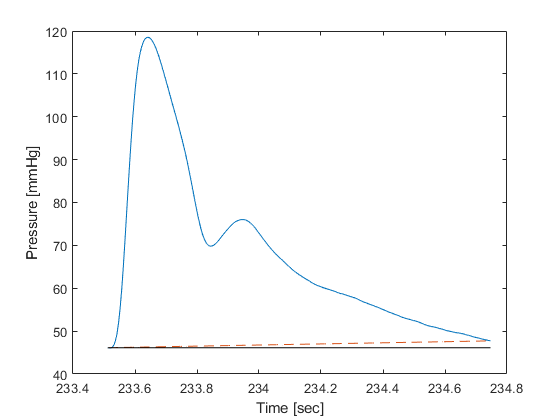
\includegraphics[width=0.45\textwidth]{fig/methods/discontinuity_signal.png}
      \label{fig:discontinuity_signal}}
      \hfill
      \subfloat[]{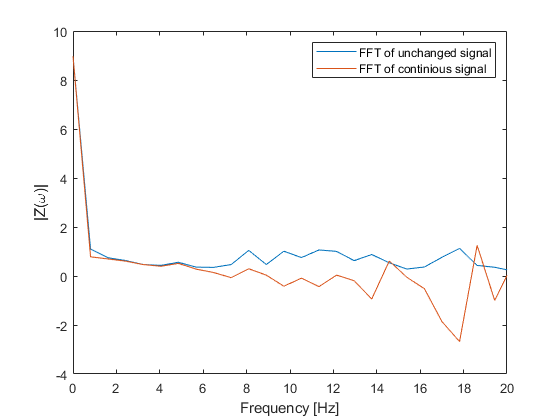
\includegraphics[width=0.45\textwidth]{fig/methods/discontinuity_dft.png}
      \label{fig:discontinuity_dft}}
  \caption{A linear function between the start and end values are used to remove the sharp transition that occurs when the measured value at the beginning and end of the cardiac cycle is different (a). This reduces the spectral leakage that would transpire as the Fourier analysis has to try to recreate the signal.}
  \label{fig:discontinuity}
\end{figure}

Usually, a window function like Hamming, Hanning, etc., are used to mitigate the effects of spectral leakage. If we were to apply such a window to our signal, it would attenuate our calculated compliance, and make it more difficult to detect changes deviations that originate from the disease. To remove the sharp transitions from one cycle to the next and reduce the effect of spectral leakage, A linear function between the start and end values, shown as the red dashed line in figure \ref{fig:discontinuity_signal}, was subtracted from the signal. Afterward, the signal, now centered around zero, was moved back to the mean value of the previous start and end value. This way, we avoid the potential of spectral leakage when there is a discontinuity between the beginning and end of the pressure and velocity measurements. Although it did not make a big difference in the specific cycle shown in figure \ref{fig:discontinuity}, it could potentially be a much larger transition, which would give rise to a more substantial amount of spectral leakage.


\section{Parameter analysis} 

Section \ref{sect:impedance} and its figure \ref{fig:impedance} introduced that the SVR is given by the 0-frequency component of the impedance, while the arterial compliance by the magnitude of the first harmonic. Afterward, section \ref{sect:modeling} gave us an analogy to a 2-element WK model and an analogy to a parallel RC circuit. The next thing we need to do is calculate the parameters for each cardiac cycle and analyze the slow oscillations caused by the autoregulation.

\subsection{Parameter estimation} \label{sect:parameter_estimation}

Figure \ref{fig:parameter_diagram} shows a simple diagram of how the parameters are extracted from a 4-minute recording. The parameters are found for every cardiac cycle of the 4-minute recording. The SVR is simply the magnitude of the 0-frequency. To find the compliance, however, a simple parametric fit is used to determine the compliance that produces the lowest error for the impedance function given in equation \ref{eq:impedance}. 

When both SVR and compliance are found for the full 4-minute measurements, they are stored as MATLAB arrays. In figure \ref{fig:parameters_patient18}, both SVR and the computed compliance are shown as a function of time. As a connection, one can take note of how both the SVR and compliance are showing the same respiratory oscillations as for the pressure and velocity. The main takeaway, however, is the presence of slow 20- to 100-second variations in all of the hemodynamic parameters. By comparing the plot of the parameters with the actual measurements in figure \ref{fig:measurements_patient18}, we can see the theory introduced in section \ref{sect:autoregulation} and figure \ref{fig:compliance_flow} concerning autoregulation in action.  As the blood pressure rises, the compliance shows an opposite trend, most likely because of the myogenic autoregulatory mechanisms altering the elasticity of the vascular smooth muscle.

\newpage

\begin{figure}[h!]
    \centering
    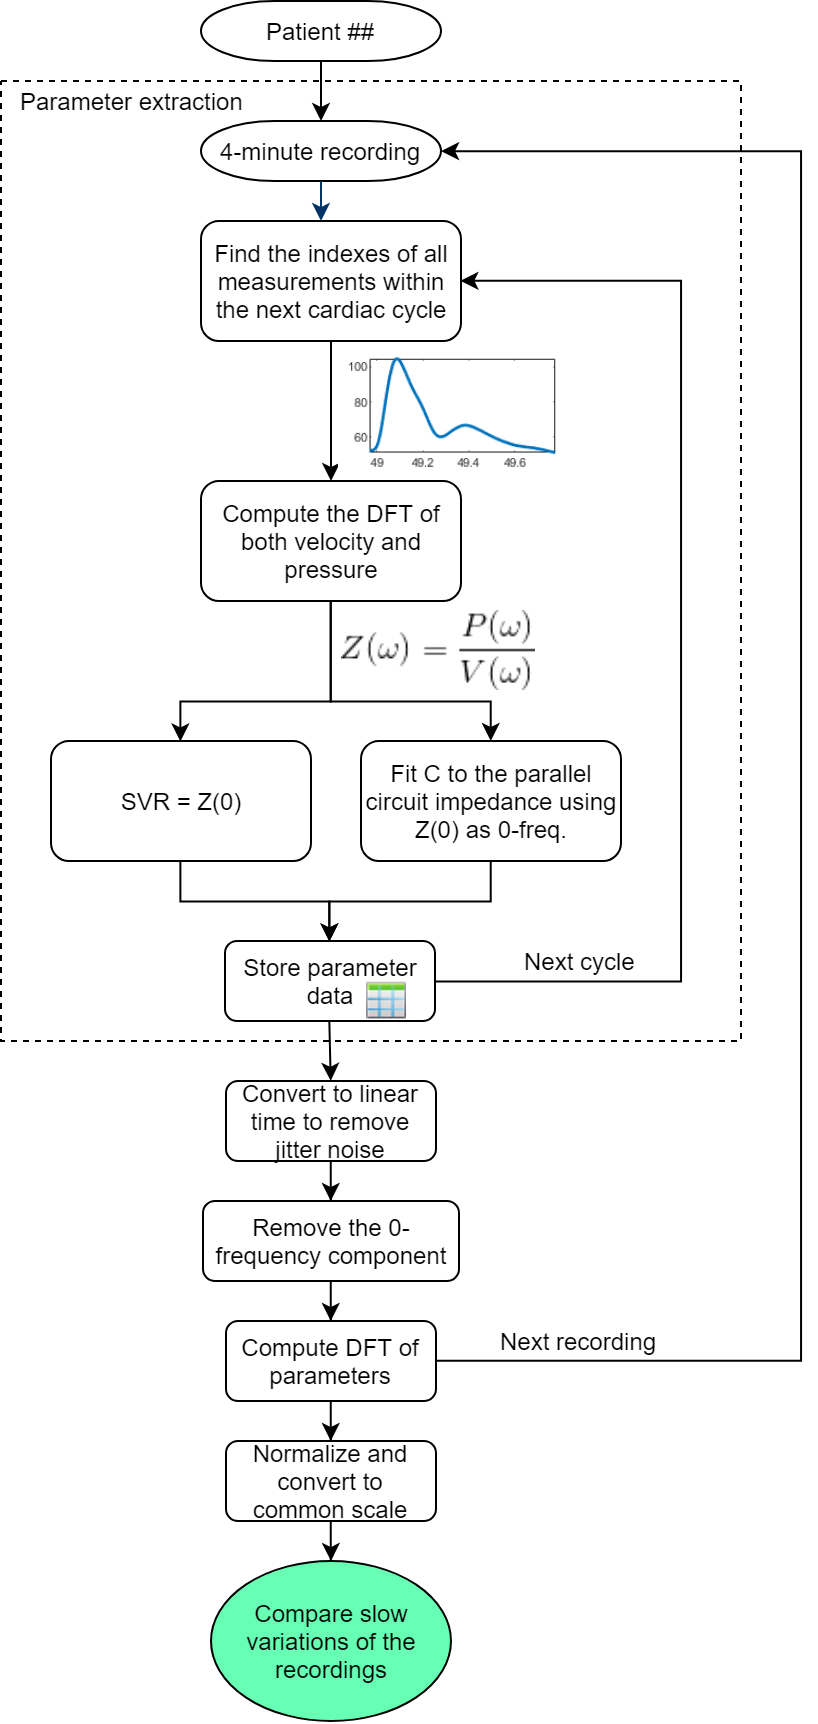
\includegraphics[width=0.6\textwidth]{fig/methods/parameter_diagram.png}
    \caption{Diagram of how the parameters are extracted from a 4-minute recording and compared to the other recordings.}
    \label{fig:parameter_diagram}
\end{figure}{}

\newpage


\newpage

\begin{figure}[b!]
    \centering
    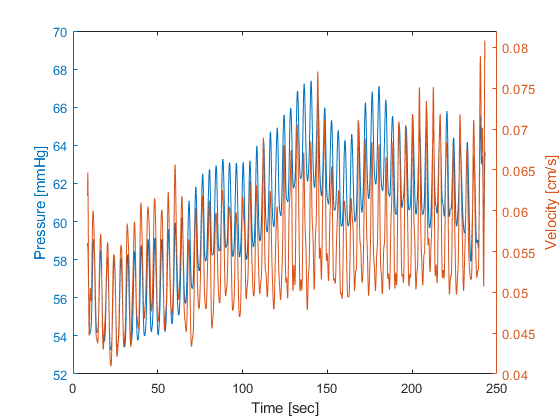
\includegraphics[width=0.75\textwidth]{fig/methods/measurements_patient18.png}
    \caption{Filtered pressure and velocity recordings. The filter is used to remove the pulmanory frequency ($\sim$1.25) and other higher frequencies such that only the changes from the respiration and the autoregulation is visible.}
    \label{fig:measurements_patient18}
\end{figure}{}

\begin{figure}[b!]
    \centering
    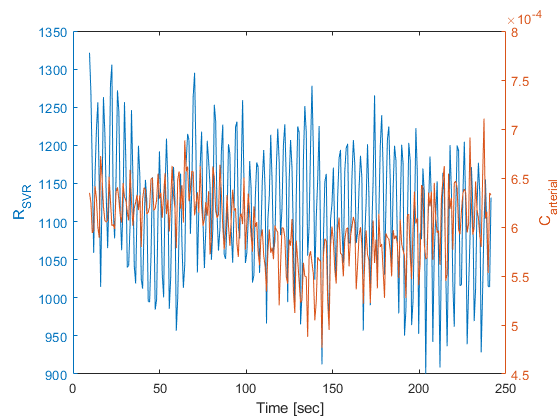
\includegraphics[width=0.75\textwidth]{fig/methods/parameters_patient18.png}
    \caption{The 2-element WK parameters calculated from the full 4-minute recordings of pressure and velocity in figure \ref{fig:measurements_patient18}. For each cardiac cycle, i.e., once every 0.6-0.8 seconds, the parameters are calculated. By comparing the slow variations of the pressure, velocity, and compliance, one can observe the autoregulation from section \ref{sect:autoregulation} and figure \ref{fig:compliance_flow} in action.}
    \label{fig:parameters_patient18}
\end{figure}{}

\newpage



\subsection{Analyzing lower frequencies}

We are now interested in analyzing the slow, autoregulatory variations of the parameters. The theory is that in the presence of a disease like sepsis, irregularities in these slow varying changes will manifest itself in the systems attempt to maintain blood perfusion through its ability to modify parameters like SVR and arterial compliance. This will cause the lower frequencies of a DFT to correlate more with the parameter signals and increase their spectral density, which we should be able to detect.

\subsubsection{Converting to linear time}

In the parameter extraction shown in figure \ref{fig:parameter_diagram}, the time indices that make up a cardiac cycle are the ones within the registered timestamps of the pulses. The pulse does not work at a constant frequency, and hence the parameter measurements performed every cardiac cycle will not have a uniform time axis. This deviation from true periodicity is registered as jitter noise in the frequency analysis. A simple fix is to interpolate the signal. The MATLAB function \texit{interp1()} was used to upsampling the signal by a factor of 10 and subsequently interpolating it using the '\texit{PCHIP}' (piecewise cubic Hermite polynomial) method.

\subsubsection{Frequency analysis}

Before finding the amplitude of the parameter's frequencies, we want to remove the 0-frequency component from the parameter data. The reason being that we are multiplying with a rectangular window as we are working with a finite number of samples, which will cause spectral leakage. The spectral leakage can be devastating for parameters of recordings with a much higher 0-frequency magnitude relative to the harmonic frequencies. When the parameters have been interpolated and had its 0-frequency component removed, the discrete-time sampled frequencies of the finite sequence of equally-spaced parameter samples are found by performing a digital Fourier transform (DFT): 
\begin{equation}
    X(k) = \frac{1}{N}\sum_{n=0}^{N-1} x(n)e^{-j(\frac{2\pi}{N})nk} 
    \label{eq:DFT}
\end{equation}
Since a DFT accumulate the amplitude of each sample for a given frequency, the magnitudes of the frequencies are normalized by a factor N-samples:

\subsubsection{Comparing the recordings} \label{sect:method_comparing_recordings}
After transforming the parameters of all the available recordings for a given patient into the frequency domain, we need to find a common scale as blood pressure and velocities can both vary on a day-to-day basis or depending on the patient has a disease like sepsis. If one parameter's mean value is much higher in one recording than the others, its variations will scale and become much higher as well, giving it seemingly the highest magnitudes. By dividing the frequency components of the parameters by its 0-frequency, we transform all of the recordings to a similar and relative scale. 

Figure 1 shows the final DFT for a random recording, which will be the basis for comparing the contribution of the parameters from the lower frequencies. As a minor validity test, one can check for the respiratory frequency at 0.25 Hz. The following chapter will compare the parameters found from the recordings of 7 patients.
\begin{figure}[h!]
    \centering
    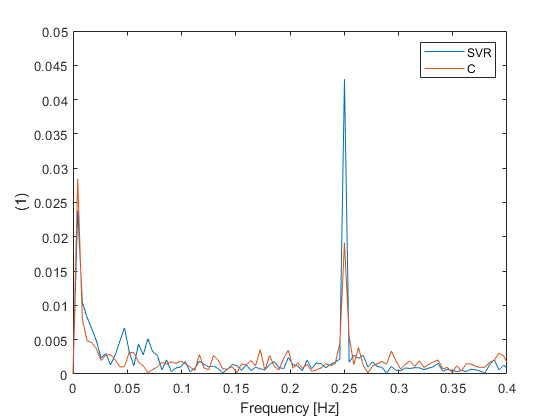
\includegraphics[width=0.75\textwidth]{fig/methods/final_dft.png}
    \caption{A sample of the final DFT of the parameters for a given recording, which will be used when comparing recordings. The y-axis is unitless relativity measure.}
    \label{fig:final_dft}
\end{figure}{}





\cleardoublepage